\documentclass[a4paper]{ctexart}
\usepackage[top=2.3cm,bottom=2cm,left=1.7cm,right=1.7cm]{geometry} 
\usepackage{amsmath} 
\usepackage{booktabs}
\usepackage{amsthm}
\usepackage{longtable} 
\usepackage{graphicx}
\usepackage{subfigure}
\usepackage{caption}
\usepackage{fontspec}
\usepackage{titlesec}
\usepackage{fancyhdr}
\def\degree{$^{\circ}$}
\def\mm{\mathrm{mm}}
\def\cm{\mathrm{cm}}
\def\nm{\mathrm{nm}}
\def\V{\mathrm{V}}
\def\m{\mathrm{m}}
\def\g{\mathrm{g}}
\def\s{\mathrm{s}}
\def\i{\mathrm{i}}
\title{\textbf{RLC电路的谐振现象}}
\author{王崇斌 1800011716}
\date{}
\makeatletter %使\section中的内容左对齐
\renewcommand{\section}{\@startsection{section}{1}{0mm}
	{-\baselineskip}{0.5\baselineskip}{\bf\leftline}}
\makeatother
\begin{document}
	\pagestyle{fancy}
	\lhead{普通物理实验报告} 
	\chead{}
	\rhead{}
	\maketitle
    \thispagestyle{fancy}
    \section{\large{实验内容与数据处理}}
    \subsection{串联谐振电路的相关实验}
    \subsubsection{用李萨如图形测量串联谐振电路的频率范围}
    \par 
    首先连接好电路,调节示波器为$x-y$模式,调节示波器上图形为一沿对角线方向延申的线段
    (这个要通过调节两个频道的电压偏转因数来实现),这样可以更加精确地观察图形是否为
    严格的线形,从而准确地判断发生谐振的频率。测得谐振怕频率范围为:$f = 2248.0\;\mathrm{Hz} \sim 2250.5\;\mathrm{Hz}$
    实验中选取$2249.0\;\mathrm{Hz}$作为谐振频率,并控制不变,在此基础上进行测量。
    \begin{table}[htbp]
        \centering
        \caption{发生谐振时的相关数据表}
        \begin{tabular}{ccccc}
            \toprule[1.5pt]
            标准电阻$R(\Omega)$ & 标准电阻两端电压$u_{R}(\V)$ & 电感两端电压$u_{L}(\V)$ & 电容两端电压$u_{C}(\V)$ & 总电压$u(\V)$\\
            \midrule
            $100 \pm 0.01$ & 1.4673 & 20.505 & 20.450 & 1.9201\\
            \bottomrule[1.5pt]
        \end{tabular}
    \end{table}
    \par 
    由于发生谐振时整个电路的阻抗为实数,根据上表数据我们可以计算电路中的电阻:
    $$
    R_{t} = \frac{u}{i} =\frac{u R}{u_{R}} = \frac{1.9201\times 100}{1.4673}\;\Omega = 130.86\;\Omega
    $$
    \par 
    由此可以得到电感在此频率下的损耗电阻$R^{'} = R_{t} - R = 30.86\;\Omega$。
    \par 
    由以上数据进一步可以计算品质因数:
    $$
    Q_{1} = \frac{\omega_{0}L}{R_{t}} = \frac{2\pi\times 2249.0 \times 0.1000}{130.86} = 10.80
    $$
    $$
    Q_{2} = \frac{u_{c}}{u} = \frac{20.450}{1.9210} = 10.65
    $$
    \par 
    我们可以进一步计算求得的品质因数的不确定度。首先讨论$Q_{1}$的不确定度。
    $$
    \sigma_{Q_{1}} = Q_{1}\sqrt{\left(\frac{\sigma_{\omega_{0}}}{\omega_{0}}\right)^{2} + 
    \left(\frac{\sigma_{L}}{L}\right)^{2} + \left(\frac{\sigma_{R_{t}}}{R_{t}}\right)^{2}}
    $$
    $$
    \sigma_{R_{t}} = R_{t}\sqrt{\left(\frac{\sigma_{U}}{u}\right)^{2} + \left(\frac{\sigma_{R}}{R}\right)^{2} + \left(\frac{\sigma_{u_{R}}}{u_{R}}\right)^{2}}
    $$
    \par 
    由元件的参数和电表的参数我们可以估计相应测量量的不确定度:
    \begin{align*}
    \sigma_{u} &= \frac{1}{\sqrt{3}}(1.9210 \times 0.2\% + 0.001)\;\V = 2.80\times 10^{-3}\;\V \\
    \sigma_{R} &= \frac{1}{\sqrt{3}} \times 0.01\;\Omega = 5.77 \times 10^{-3}\;\Omega \\
    \sigma_{u_{R}} &= \frac{1}{\sqrt{3}} \times (1.4673 \times 0.2\% + 0.001)\;\Omega = 2.27 \times 10^{-3}\;\Omega \\ 
    \sigma_{\omega_{0}} &= \frac{1}{\sqrt{3}}(2250.5-2248.0)\mathrm{Hz} = 1.44\mathrm{Hz}\\
    \sigma_{L} &= \frac{1}{\sqrt{3}} 0.1\times 0.1\% \mathrm{H} = 5.77\times 10^{-5}\mathrm{H}
    \end{align*}
    \par 
    将上面的数据带入公式可以得到:
    $$
    \sigma_{R_{t}} = 0.28\;\Omega
    $$
    $$
    \sigma_{Q_{1}} = 0.02
    $$
    \par 
    由此可以写出$Q_{1} = 10.80 \pm 0.02$
    \par 
    容易的到$Q_{2}$的不确定度表达式为:
    $$
    \sigma_{Q_{2}} = Q_{2}\sqrt{\left(\frac{\sigma_{u_{C}}}{u_{C}}\right)^{2} + \left(\frac{\sigma_{u}}{u}\right)^{2}}
    $$
    $$
    \sigma_{U_{C}} = \frac{1}{\sqrt{3}}(20.450 \times 0.2\% + 0.01)\;\V = 0.051\;\V
    $$
    $$
    \sigma_{Q_{2}} = 0.03
    $$
    \par 
    因此$Q_{2} = 10.65 \pm 0.03$\\
    \subsubsection{测量RLC电路的相频特性}
    \par 
    本实验中测量电流与电压相位差的方法是通过示波器测量电路两端的总电压与标准电阻两端的电压相位差
    ,由于纯电阻元件不会改变相位,这样就测得了电路中电压与电流之间的相位差。将实验中改变
    频率测得的相位差数据列表如下:
    \begin{table}[htbp]
        \centering
        \caption{串联谐振电路电压与电流之间相位差与信号源频率关系的实验数据表}
        \begin{tabular}{cccc}
            \toprule[1.5pt]
            频率$f(\mathrm{kHz})$ & 时间差$\Delta t(\mathrm{ms})$ & 相位差$\phi(^{\circ})$\\
            \midrule
            1.7490 & -0.129 & -81.2 \\
            1.9550 & -0.1020 & -71.8 \\
            2.0850 & -0.0795 & -59.7 \\
            2.1500 & -0.0588 & -45.5 \\
            2.1940 & -0.0376 & -29.7 \\
            2.2220 & -0.0214 & -17.1 \\
            2.2495 & 0       & 0     \\
            2.2780 & 0.0202 & 16.6\\
            2.3110 & 0.0364 & 30.3\\
            2.3550 & 0.0542 & 45.95\\
            2.4360 & 0.0680 & 59.6\\
            2.8590 & 0.0770 & 71.8\\
            2.9090 & 0.0748 & 78.3\\
            \bottomrule[1.5pt]
        \end{tabular}
    \end{table}
    \par 
    上面表格给出的相位差由下式算出:
    $$
    \phi = \Delta t f \times 360\;^{\circ}
    $$
    \par 
    由理论知识我们可以得到相位差的理论表达式为:
    $$
    \phi = \arctan\frac{\omega L - \frac{1}{\omega C}}{R}
    $$
    \begin{figure}[htbp]
        \centering
        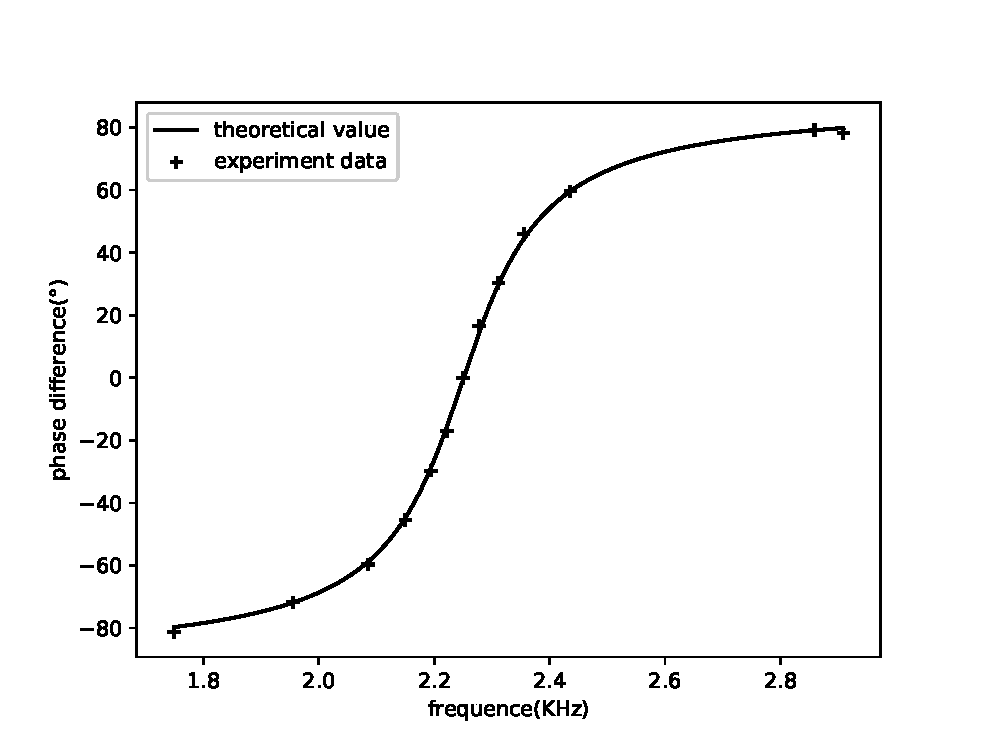
\includegraphics[scale=0.75]{phase.eps}
        \caption{相移曲线的实验值与理论值对比}        
    \end{figure}
    \par 
    从图中可以看出,实验值与理论值符合得相当好。\\
    \subsubsection{测量RLC电路的幅频特性}
    \par 
    测量的基本方法是通过测量标准电阻两端的电压来计算串联电路中的电流,得到电流随信号源频率
    的变化关系。
    \begin{table}[htbp]
        \centering
        \caption{标准电阻两端电压随信号源频率的变化关系}
        \begin{tabular}{ccc|ccc}
            \toprule[1.5pt]
            $f(\mathrm{kHz})$ & $u_{R}(\V)$ & $i(\mathrm{mA})$ & $f(\mathrm{kHz})$ & $u_{R}(\V)$ & $i(\mathrm{mA})$\\
            \midrule
            1.7490 & 0.1370 & 1.370 & 2.2495 & 0.7616 & 7.616 \\
            1.8000 & 0.1543 & 1.543 & 2.2600 & 0.7561 & 7.561 \\
            1.9550 & 0.2398 & 2.398 & 2.2780 & 0.7310 & 7.310 \\
            2.0000 & 0.2871 & 2.871 & 2.2900 & 0.7058 & 7.058 \\
            2.0850 & 0.4185 & 4.185 & 2.3100 & 0.6548 & 6.548 \\
            2.1200 & 0.4757 & 4.757 & 2.3400 & 0.5746 & 5.746 \\
            2.1500 & 0.5505 & 5.505 & 2.3500 & 0.5367 & 5.367 \\
            2.1700 & 0.6080 & 6.080 & 2.4000 & 0.4400 & 4.400 \\
            2.1940 & 0.6769 & 6.769 & 2.4360 & 0.3816 & 3.816 \\
            2.2000 & 0.6928 & 6.928 & 2.7000 & 0.1861 & 1.861 \\
            2.2220 & 0.7371 & 7.371 & 2.8590 & 0.1430 & 1.430 \\
            2.2400 & 0.7602 & 7.602 & 2.9090 & 0.1336 & 1.336 \\
            \bottomrule[1.5pt]
        \end{tabular}
    \end{table}
    \par 
    我们有电路中电流大小的理论公式:
    $$
    i = \frac{u}{\sqrt{R^{2} + \left(\omega L - \frac{1}{\omega C}\right)^{2}}}
    $$
    \par 
    根据上式我们画出实验数据点与理论的曲线进行比较:
    \begin{figure}[htbp]
        \centering
        \includegraphics[scale=0.75]{amplitude.eps}
        \caption{幅频曲线的实验值与理论值对比}
    \end{figure}
    \par 
    可以看出实验值与理论值非常吻合。考虑电压为$\frac{u_{R}}{\sqrt{2}}$时对应的频率,通过
    这两个频率之差来计算品质因数$Q_{3}$。$\frac{u_{R}}{\sqrt{2}} = 0.5385 \;\V$,实验中
    测量了如下两个数据点$(0.5389\;\V,\;\;2354.0\mathrm{Hz}),\;\;(0.5380\;\V,\;\;2145.5\mathrm{Hz})$。
    $$
    Q_{3} = \frac{f_{0}}{\Delta f} = 10.79
    $$\\
    \subsubsection{测量黑盒子中的元件参数}
    \par 
    本实验中测量的黑盒子中含有电感、电阻、电容中的两种元件,实验思路是首先通过谐振发生的条件
    判断盒子中元件的种类,再根据谐振时的各种参数确定盒子中元件的参数。实验时选取了10号盒子。
    \par 
    首先单独将X与标准电阻接入电路,不断改变信号源频率观察示波器上电阻两端电压与总电压的相位差
    变化,发现相位差没有变化,说明盒子中的两个元件不能发生谐振,因此只有电感或者电容中的一种。
    进一步将X与电容和电感分别串联,观察在改变信号源频率时是否有谐振发生。实验发现在与电容
    串连时可以发生谐振,因此确定了10号盒子中含有电感。
    \par
    改变标准电容的大小,记录发生谐振时的信号源频率,得到如下数据表:
    \begin{table}[htbp]
        \centering
        \caption{串联谐振频率随电容的变化数据表}
        \begin{tabular}{cccc}
            \toprule[1.5pt]
            $C(\mu F)$ & 0.05 & 0.10 & 0.15\\
            \midrule
            $f(\mathrm(kHz))$ & 7.21 & 5.09 & 4.18 \\
            \bottomrule[1.5pt]
        \end{tabular}
    \end{table}
    \\
    可以根据谐振发生的条件得到电感的表达式:
    $$
    L = \frac{1}{C} \times \frac{1}{(2\pi f)^{2}}
    $$
    \par 
    求得电感的平均值为$\bar{L} = 9.73 \times 10^{-3}\;\mathrm{H}$
    \par 
    在谐振时测量标准电阻两端电压与总电压为:$u_{R} = 0.1258\;\V.\;\; U_{t} = 1.4156\;\V$
    由此可以计算出盒子中的总电阻(包含了电感的损耗电阻)$R_{0} = \frac{u_{t}}{u_{R}}\times 100 - 100 = 1025.3 \;(\Omega)$
    与10号盒子的真实数据$(L = 9.791 \;\mathrm{mH},\;\;R^{'} = 23.24\;\Omega,\;\; R = 1000\;\Omega)$
    ,可以看到我们的测量结果还是比较接近的。\\
    \\
    \section{\large{思考题}}
    \paragraph{(1)} 
    首先我们观察一下决定谐振特性的相关公式:
    $$
    \phi = \arctan\frac{\omega L - \frac{1}{\omega C}}{R}
    $$
    $$
    i = \frac{u}{\sqrt{R^{2} + \left(\omega L - \frac{1}{\omega C}\right)^{2}}}
    $$
    $$
    Q = \frac{\omega_{0}L}{R}
    $$
    可以看到将标准电阻的阻值改变不会影响到谐振频率,但是会影响到谐振幅频特性与品质因数。
    $i_{m}^{'} = \frac{130.86}{530.86}i_{m},\;\;Q^{'} = \frac{130.86}{530.86}Q$。
    可以通过画图来对比幅频曲线的差异:
    \begin{figure}[htbp]
        \centering
        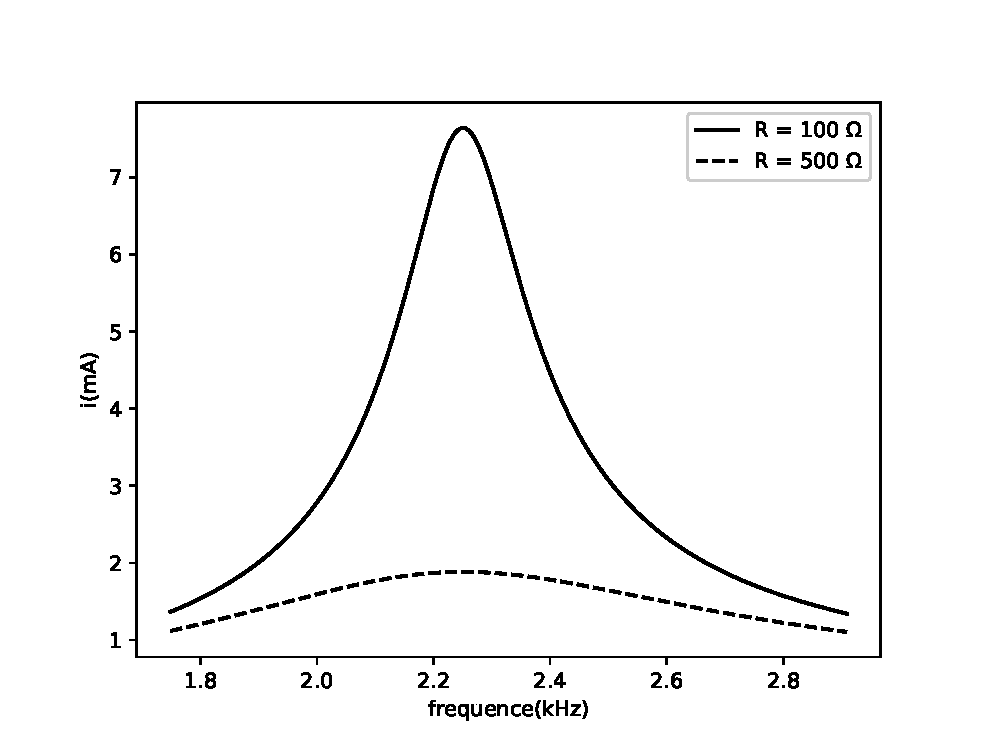
\includegraphics[scale=0.8]{compare.eps}
        \caption{两种阻值下幅频曲线的差异}
    \end{figure}
    \par 
    可以看出当标准电阻的阻值增大后,幅频曲线已经不再是典型的谐振电路的幅频曲线了,变得非常
    平滑,此时品质因数很小,电路的储能效率与选频特性十分低下,这提醒我们在设计谐振电路时
    有必要控制损耗电阻的大小。
    \paragraph{(2)}
    \par
    测量原理与测量步骤:将待测元件接入电路,调节可变电容使得电路发生谐振,测量此时的总电压$u$,
    可变电容两端的电压$u_{C}$,可以计算出:
    \begin{align*}
        Q &= \frac{u_{C}}{u}\\
        L &= \frac{1}{C} \times \frac{1}{(2\pi f)^{2}}\\
        r &= \frac{1}{2\pi f Q C}\\
    \end{align*}
    \par 
    这样就可以计算出题目中的数据:
    \begin{align*}
        Q &= 100\\
        L &= 2.13 \times 10^{-4}\;\mathrm{H} \\
        r &= 8.04\;\Omega\\
    \end{align*}
    \\
    \section{\large{分析与讨论}}
    \par 
    可以看到通过谐振频率与通频带宽计算出来的$Q_{1},\;\;Q_{3}$几乎
    完全一致,而通过总电压与电容电压的比值计算出来的$Q_{2}$略微偏小
    我觉得这有可能是电路之间的分布性电容分掉了标准电容的电压,导致
    测量到的电容电压偏小。\\
    \\
    \section{\large{收获与感想}}
    \par 
    我总觉得自己的电学实验做得不太好,面对复杂连接的导线我的心情可能比
    导线还复杂,总是得手忙脚乱一会儿,无论我在电路图上把它们看得如何清楚。
    所以在做这次实验时做的也比较慢,一下子面对这么多复杂的仪器一时不知所措,
    不过后来在测量了几组数据之后也就渐渐熟悉了。在写前面的报告时看见自己的
    数据与理论曲线很是接近,心里还挺开心的!
\end{document}